%-----------------------------------------------------------------------------
%
%               Template for sigplanconf LaTeX Class
%
% Name:         sigplanconf-template.tex
%
% Purpose:      A template for sigplanconf.cls, which is a LaTeX 2e class
%               file for SIGPLAN conference proceedings.
%
% Guide:        Refer to "Author's Guide to the ACM SIGPLAN Class,"
%               sigplanconf-guide.pdf
%
% Author:       Paul C. Anagnostopoulos
%               Windfall Software
%               978 371-2316
%               paul@windfall.com
%
% Created:      15 February 2005
%
%-----------------------------------------------------------------------------


\documentclass[preprint]{sigplanconf}

% The following \documentclass options may be useful:
%
% 10pt          To set in 10-point type instead of 9-point.
% 11pt          To set in 11-point type instead of 9-point.
% authoryear    To obtain author/year citation style instead of numeric.

\usepackage{amsmath}
\usepackage{pgfplots}
\usepackage{listings}
\usepackage{tikz}
\usetikzlibrary{positioning}

\begin{document}

\lstset{language=C++}

\conferenceinfo{WXYZ '05}{date, City.} 
\copyrightyear{2005} 
\copyrightdata{[to be supplied]} 

%\titlebanner{banner above paper title}        % These are ignored unless
%\preprintfooter{short description of paper}   % 'preprint' option specified.

\title{Reducing Software Transactional Memory Instrumentation through Memory Reservations}

\authorinfo{Gaurav Jain}
{University of Waterloo}
{gjain@uwaterloo.ca}
\authorinfo{Patrick Lam}
{University of Waterloo}
{p.lam@ece.uwaterloo.ca}

\maketitle

\begin{abstract}

%TODO read write load store
%parapgrph spacing
Software Transactional Memory abstracts the intricate complexities of concurrent programming. Though many STM libraries exist, they require manual instrumentation of memory reads and writes performed within a transaction. This needs to be carefully and selectively crafted by application developers to avoid unnecessary calls to the STM library, thus diminishing the appeal of STM. An open research topic is how compilers could automatically insert instrumentation and perform necessary optimizations. Current compiler-generated implementations perform poorly when compared to developer instrumented code~\cite{Cascaval:2008:STM:1454456.1454466}.

We propose an extension to the current API between compilers and STM libraries with \emph{memory reservations}. A memory reservation allows a transaction to specify the memory locations that will be accessed and alleviates the role of version management from the library. This technique enables the compiler to apply static analysis techniques to reduce the instrumentation required to support STM. This is especially crucial in unmanaged languages where overhead must be kept to a minimum.

\end{abstract}

\section{Background \& Introduction}

Current compiler instrumentation identifies reads and writes to shared memory locations and replaces them with calls to \verb+stm_read+ and \verb+stm_write+ respectively. Through these calls the STM library is responsible for conflict resolution and version management. If there is no conflict present, it returns the value stored in the requested memory location or writes the new value. Depending on the algorithm this may involve lookups in internal data structures and executing any necessary memory barriers. By instrumenting every read and write, the compiler is unaware of whether the writes are buffered until commit/abort or if they are written in-place. Thus some algorithms are able to exploit more concurrency through buffered writes. However this limits the scope of certain compiler optimizations as all reads and writes must be replaced with function calls. One such example, is the inability to reorder the reads and writes or cache values in registers.

Listing \ref{listing1} illustrates a functions \verb+foo()+ and \verb+bar()+ called within a transaction. A compiler would process these functions by creating clone of \verb+foo()+ and \verb+bar()+ and generate code similar to listing \ref{listing2}.

\begin{figure}[h]
\begin{lstlisting}[caption={Example},label=listing1,captionpos=b]
int a,b,c,d;

int bar(int& x) {
    return x+1;
}

int foo() {
    a = 2;
    b = 2;
    if (d > 0) {
        b = c;
    } else {
        a = bar(b);
    }
    return a + b;
}
\end{lstlisting}
\end{figure}
\noindent

\begin{figure}[h]
\begin{lstlisting}[caption={Standard STM instrumentation},label=listing2,captionpos=b]
int a, b, c, d;

int __TX_bar(int& x) {
    return stm_read(&x)+1;
}

int __TX_foo() {
    stm_write(&a, 2);
    stm_write(&b, 2);
    if (stm_read(&d) > 0) {
        stm_write(&b, stm_read(&c));
    } else {
        stm_write(&a, __TX_bar(b));
    }
    return stm_read(&a) + stm_read(&b);
}
\end{lstlisting}
\end{figure}

Our approach inserts the calls to \verb+stm_reserve+ before each shared memory access, leaving reads and writes untouched. This memory reservation requests the STM library to perform any conflict resolution and barrier operations to prevent other transactions from performing conflicting accesses. Further details of memory reservations are described in Section 2. The \verb+stm_reserve+ API supports coalescing of requests such that multiple memory addresses can be reserved in a single call, resulting in the transformation seen in listing \ref{listing3}.

\begin{figure}[h]
\begin{lstlisting}[caption={STM instrumentation with memory reservations},label=listing3,captionpos=b]
int a, b, c, d;

int bar(int& x) {
    stm_reserve(0b0, &x);
    return x+1;
}

int foo() {
    stm_reserve(0b110, &a, &b, &d);
    a = 2;
    b = 2;
    if (d > 0) {
        stm_reserve(0b10, &b, &c);
        b = c;
    } else {
       int tmp = bar(b);
       stm_reserve(0b1, &a);
       a = tmp;
    }
    stm_reserve(0b00, &a, &b);
    return a + b;
}
\end{lstlisting}
\end{figure}

Memory reservations reduce the number of calls to the STM library. In addition, since individual reads and writes are not transformed to function calls, function cloning is not required and the scope for compiler optimizations greatly increases.

The main contribution of this paper is a description of the semantics of memory reservations for unmanaged languages and the instrumentation optimizations that it enables. Section 2 describes the operation of memory reservations. Section 3 presents a compiler instrumentation pass designed for memory reservations. Section 4 evaluates the effectiveness of the approach. Section 5 describes related work, followed by conclusions in section 6.

\section{Memory Reservations}

A transaction performs reads and writes to memory on the assumption that it is isolated from the rest of the system. The STM library enables multiple transactions to execute alongside one another as long as it can ensure that there exists a serial ordering of transactions that performs the same operations. As a result, multiple transactions may share memory locations within their active working set, given that they do not conflict with one another. If a transaction begins by writing to memory location A, and a second transaction reads location A, it is possible to execute both transactions concurrently as long as the first transaction perform no further updates to A and commits before the second. If the first transaction aborts or the second transaction writes to a location read by the first, then one or both of them may need to be aborted.

Memory reservations remove the memory versioning responsibility from the STM library, such that it only needs to focus on conflict management and memory barrier calls. A \verb+stm_reserve+ call takes as its parameters a list of memory addresses and a bit vector representing whether the reservation is for read or write. If the STM library uses a global version number similar to TML\cite{Dalessandro:2010:TML:1885276.1885279}, the library can ignore the memory addresses and only look at the bit vector to search for the presence of a write reservation. Algorithms that have a more sophisticated conflict resolution policy will have to process the reservations in the order in which they are specified, to dispatch the correct action. If all the reservations in a call cannot be fulfilled, the transaction is either stalled or aborted. This motivates the compiler to request reservations as early as possible to detect conflicts earlier.

There are two types of reservations that can be requested:

\begin{itemize}

\item When a \emph{read reservation} is requested from the STM library, it ensures that the memory will be unmodified for the duration of the transaction. As a result, subsequent read reservations by the transaction to the same memory location are redundant and should be avoided. Ideally the location is not in the write set of any active transaction. If it is, the STM library may stall or abort the reader transaction. Another alternative is allow the transaction to proceed, however delay the commit until the writer has committed.

\item A \emph{write reservation} ensures that a transaction will have exclusive write access to a memory location until it commits. Thus following read and write reservations by the transaction on the memory location have no effect and are considered redundant. If an in-progress transaction has already read the memory location the writer may need to stall until the transaction has either committed or aborted. Note that it is possible for a transaction to upgrade a read reservation to a write reservation.

\end{itemize}

Listing \ref{listing4} shows the effect of removing redundant read and write reservations from listing \ref{listing3}. Removing redundant calls reduces the number of memory barriers incurred which is a form of over-instrumentation\cite{Yoo:2008:KTS:1378533.1378582}.

\begin{figure}[h]
\begin{lstlisting}[caption={Reducing redundant memory reservations},label=listing4,captionpos=b]
int a, b, c, d;

int bar(int& x) {
    return x+1;
}

int foo() {
    stm_reserve(0b110, &a, &d, &b);
    a = 2;
    b = 2;
    if(d>0) {
        stm_reserve(0b0, &c);
        b = c;
    } else {
        int tmp = bar(b);
        tmp = a;
    }
    return a + b;
}
\end{lstlisting}
\end{figure}

Compilers instrument functions called within a transaction by cloning the function. Thus an executable contains two versions of the same function, one for regular execution and the other for use within transactions. By utilizing in-place reads and writes, memory reservations can be applied to a function without the need to clone it. The \verb+stm_reserve+ call can detect that it is being executed outside of a transaction and if so, do nothing. This makes processing of function pointers much simpler as all the functions in the MAY alias set can be instrumented with limited impact.

\section{Compiler Pass Design}

We have implemented our compiler instrumentation as a LLVM\cite{1281665} pass that operates on LLVM IR bit-code generated by the clang C/C++ front-end. The pass is divided into the following 5 stages:

\begin{itemize}

\item {\bf Analysis:} The initial analysis stage identifies the functions called within a transaction and iterates each instruction to determine whether a reservation is needed. If so, a \emph{reservation site} is created for the instruction. These include memory read and write instructions as well as any atomic memory instructions. For each function call encountered, the function is added to the work queue for analysis. Additionally, function call sites are tracked for use in the forward analysis in the compression stage.

\item {\bf Compression:} The goal of this stage is to remove any reservation sites that represent a redundant reservation as described earlier. Using a inter-procedural forward analysis, each reservation site is inspected to determine if the memory location has already been read reserved or write reserved. In order for this analysis to be effective, the MUST alias analysis set is considered. Further, the forward analysis only inspects paths that are feasible within a transaction. Thus the function call sites identified in the Analysis stage are utilized to correctly traverse the call graph.To eliminate a reservation, it must be classified as a redundant call on all possible program paths. A reminder that a write reservation cannot be omitted due to a previous read reservation.

Additionally the compression stage removes reservation sites where the memory is allocated on the stack or from the heap during a transaction. Heap memory allocated within a transaction is considered private until the transaction commits.

\item {\bf Elimination:} The elimination pass attempts to remove any reservation sites generated as a result of over-instrumentation. Using a conservative MAY alias analysis, if a pointer and its MAY alias set is never written to within any transaction, all associated reservations can be removed. This supports the \emph{not-accessed-in-transaction} analysis described by Shpeisman et al.~\cite{Shpeisman:2007:EIO:1250734.1250744}. Writing to the MAY alias set outside of a transaction is still considered valid. Given strong isolation constraints, it is the responsibility of the developer to ensure that no conflicting transactions are executing during the write.

\item {\bf Merge:} Up until this stage all the reservation sites consist of a single read or write. To reduce SRM overhead, the merge stage attempts to consolidate multiple reservations. Similar to the compression stage, a forwards analysis is run on each reservation site to see if there exists an earlier site for each program path. Once it has been determined that the necessary conditions are met, the reservation site is removed and merged with each of the previous sites. The merge ensures that the ordering of reservations is preserved.

\item {\bf Instrumentation Phase:} Finally the instrumentation stage inspects the remaining non-empty reservations sites and constructs a call to \verb+stm_reserve+.

By dividing the pass into these 5 stages, we were able to identify the benefits of each optimization in our evaluation.

\end{itemize}

\subsection{MAY Alias Analysis}

The elimination stage relies heavily on the MAY alias analysis. We employ a conservative analysis that is efficiently able to compute a MAY alias set. If a MAY alias set for a pointer cannot be determined the elimination stage is skipped.

An important property of the MAY alias set is that it need not be precise. However the MUST alias set must be a subset of the MAY alias set. This ensures that the elimination analysis is sound. The alias analysis cannot restrict itself to only instructions executed in a transaction. Doing so could loose important MAY alias information. An example of this would be an object where member pointer are initialized in the constructor. If the object is constructed outside a transaction and subsequently used within a transaction, the alias analysis would miss information obtained from analyzing the constructor.

The analysis iterates through each program instruction and creates a relationship map for each value it encounters. A value could be a global, function parameter, stack variable, register or memory location. The map consists of 4 types of relations:

\begin{itemize}

\item {\bf Alias:} If a value is a function parameter each of the function call sites of the function is examined and the value passed in as a parameter by the caller is aliased to parameter value. Any incoming values to a PHI node are aliased with each other as well as the PHI node. Additionally, any cast or selection operations result in an alias relationship. The Alias relationship is bidirectional, i.e. it is added to the relationship map of both pairs.

\item {\bf Loaded From/By:} For values that are read from memory locations specified by other values, a \emph{Loaded From} relation is added. The value storing the memory location has a \emph{Loaded By} relation added to it's map.

\item {\bf Store From/Into:} For values that are written into locations pointed to by other values, a \emph{Stored Into} relation is added. A \emph{Store From} relation is added to the value being dereferenced and written into.

\item {\bf Offset Parent/Child:} The LLVM subsystem supports indexing of object members through the \verb+GetElementPtr+ instruction. If a value is generated as a result of a \verb+GetElementPtr+ it adds an \emph{Offset Parent} relationship with the operand value and correspondingly a \emph{Offset Child} relationship. Additionally the \verb+GetElementPtr+ offset calculation is recorded to distinguish between different child values. Note that any value can only have a single parent relationship, while a parent may have many offset children.

\end{itemize}

When a MAY alias set is requested for a value, the algorithm recursively iterates through all the Alias relations and adds their MAY alias sets. If the value has a Loaded From relation, the Loaded By children from the MAY alias set of the loaded value are added. Furthermore, if any of the loaded MAY alias values have a Stored From relation, those aliases are added as well. If a value has a stored into value, any values that are loaded from that value are considered aliases.

If a value has an Offset Parent relationship, all the relationship maps are iterated over to find offset children that have the same \verb+GetElementPtr+ calculation. If the calculation matches, the child value is added to the MAY alias set. Note that the parents are not queried as to whether they alias to each other. This approach is an over approximation of the MAY alias set. However it is more efficient than traversing through the offset parent and children relationships and our results show that it is still quite effective.

It possible that a while computing the MAY alias set a recursive relationship is found, such as a value aliasing to its Loaded From alias set. This is not uncommon for linked data structures such as lists and trees. If such a condition is met we cannot safely compute a MAY alias set. Similarly, since our alias analysis requires whole program analysis, if any of the traversals leads to values used in external library calls, we cannot compute a valid alias set.

\section{Evaluation}

\subsection{Instrumentation Overhead}

To evaluate the effectiveness of our approach, we applied our compiler pass to the \verb+vacation+ benchmark from the STAMP~\cite{4636089} suite. This benchmark emulates a travel reservation system which uses software transactions to concurrently modify a red black tree. As a result, most of the application workload executes within a transaction. We compare the compiler instrumented code generated at various stages against manually instrumented code by running the benchmark and recording the number of read and write reservations.

The manual instrumentation resulted in code that issued 12,357 write calls. Using only the analysis stage,  the compiler instrumented code issued 28,066 write reservations. Applying the compression stage brought the compiler instrumentation in line with the manual instrumentation. Closer inspection showed all of the excessive write calls to be stack or thread-local heap allocations. Further passes were not able to reduce the number of write operations, however we did observe that not all 12,357 writes were to unique memory locations. Our analysis could not perform better than the manually instrumented code since the memory locations were dynamically calculated could not be aliased statically.

\begin{figure}
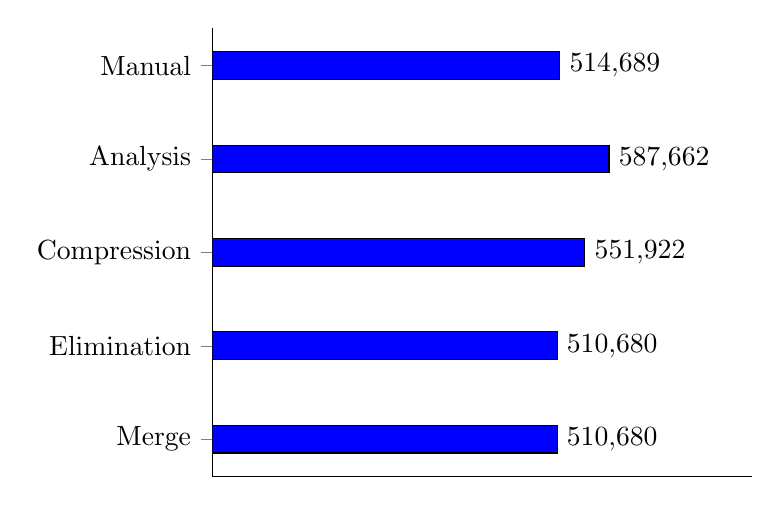
\begin{tikzpicture}
    \begin{axis}[%
            /pgf/number format/.cd,
            fixed,
            precision=0,
            xbar,
            symbolic y coords={Merge,Elimination,Compression,Analysis,Manual},
            nodes near coords={\pgfmathprintnumber\pgfplotspointmeta},
            nodes near coords align={horizontal},
            xtick=\empty,
            axis x line*=bottom,
            axis y line*=left,
            xmin=0,
            xmax=800000,
        ]
        \addplot[fill=blue] coordinates {
            (514689,Manual)
            (587662,Analysis)
            (551922,Compression)
            (510680,Elimination)
            (510680,Merge)
        };
    \end{axis}
\end{tikzpicture}
\caption{Read instrumentation function calls}\label{marker1}
\end{figure}

Figure \ref{marker1} shows the number of read calls issued from code generated after each stage. With reads, the compression pass was not sufficient to bring the instrumentation in line with the manual results. However the elimination pass was able to reduce the overhead beyond what the manual method was able to achieve. Besides removing reservations to read-only memory locations this improvement is largely due to the \emph{not-accessed-in-transaction}~\cite{Shpeisman:2007:EIO:1250734.1250744} analysis. We found that manual instrumentation was conservative with reads in certain library routines. Compiler analysis was able to deem those reads a unnecessary due to the locations never being written to within a transaction.

From statistics gathered, there were 121 reservation sites which reserved a 1 pointer location and 7 which reserved 2 locations. Figure \ref{marker2} demonstrates that due to the large percentage of reservation sites consisting of a single pointer location the merge stage could only reduce the total of library calls by 1\% from the elimination stage. This resulted in an overall improvement of 1.6\% when compared to manual instrumentation. We believe that this can be improved if we apply techniques to safely apply loose ordering.

\begin{figure}
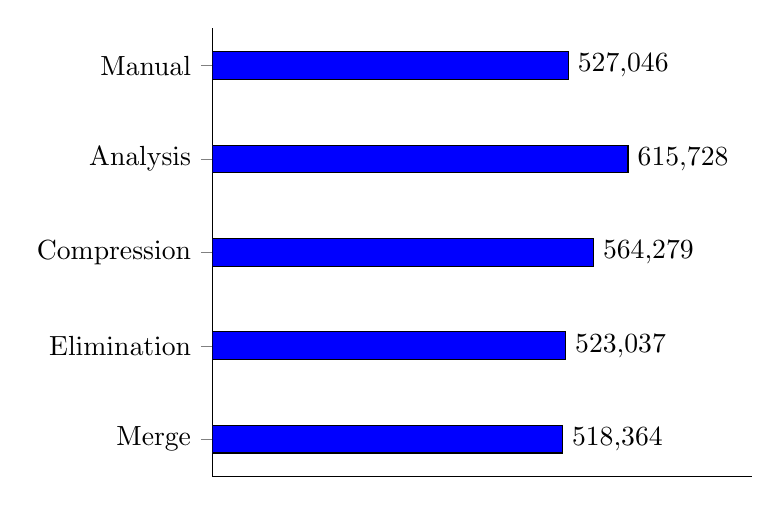
\begin{tikzpicture}
    \begin{axis}[%
            /pgf/number format/.cd,
            fixed,
            precision=0,
            xbar,
            symbolic y coords={Merge,Elimination,Compression,Analysis,Manual},
            nodes near coords={\pgfmathprintnumber\pgfplotspointmeta},
            nodes near coords align={horizontal},
            xtick=\empty,
            axis x line*=bottom,
            axis y line*=left,
            xmin=0,
xmax=800000,
        ]
        \addplot[fill=blue] coordinates {
            (527046,Manual)
            (615728,Analysis)
            (564279,Compression)
            (523037,Elimination)
            (518364,Merge)
        };
    \end{axis}
\end{tikzpicture}
\caption{Total instrumented function calls}\label{marker2}
\end{figure}

\section{Related Work}

Wang et al~\cite{4145103} were the first to describe techniques to enable compiler support of STM in unmanaged languages. Our approach builds on this work, but limits the range of STM algorithms to enable better compiler optimizations. As a result, we can avoid the need to clone functions and are able to support function pointers with far greater ease than what has been previously proposed.

TANGER~\cite{felber2007tanger} did similar work on LLVM to support STM in unmanaged languages. Additionally it utilized TARIFA to support binary translation of non-instrumented code. Without binary translation, it was able to match the performance of hand-instrumented code. These were positive results, however it is not enough. Manually instrumented code does not achieve the scalability of fine-grained locking alternatives. Thus it is not sufficient to match it's performance, compilers need to be able to do far better. We believe our approach leads towards this goal.

TML\cite{Dalessandro:2010:TML:1885276.1885279} presents an adaptation of STM whereby it allows multiple readers and a single writer. Once a writer acquires the lock, ongoing reader transactions are aborted. Since no other transactions are active while a writer is in progress, instrumentation after the first write can be omitted. The use of memory reservations does not preclude this optimization, however a single writer model may not be optimal. Further static analysis may enable multiple writers to execute simultaneously.

\subsection{Performance}

To evaluate the performance of reservations we utilized the RSTM transactional memory library and modified 3 in-place write algorithms; TML, OrecEager (which resembles TinySTM~\cite{Felber:2008:DPT:1345206.1345241}) and ByteEager (resembling TLRW~\cite{Dice:2010:TRR:1810479.1810531}).

\section{Conclusions \& Future Work}

There is a strong desire to use STM as a means of efficiently enabling concurrent access to complex data structures and program logic. Restricting the role of an STM library to only conflict management enables the compiler to apply optimizations that may not be otherwise feasible. The use of memory reservations with alias analysis is able to reduce the overhead associated with STM instrumentation beyond what is possible through manual methods.

Further use of static analysis can assist in reducing the overhead of STM. Our current compiler implementation focuses on static analysis to limit compiler instrumentation. We plan to implement analysis that may assist the conflict management of the STM library as well. Knowledge of whether a transaction is read-only or whether it can initiate an abort may allow the conflict resolution to take a much more efficient approach. Additional analysis to describe whether writer transactions are non-conflicting may enable more concurrency.

\appendix

% We recommend abbrvnat bibliography style.
%{\footnotesize \bibliographystyle{abbrvnat} \bibliography{sigplanconf-template}}
\bibliographystyle{abbrvnat}

% The bibliography should be embedded for final submission.

\begin{thebibliography}{10}
\softraggedright
\providecommand{\natexlab}[1]{#1}
\providecommand{\url}[1]{\texttt{#1}}
\expandafter\ifx\csname urlstyle\endcsname\relax
  \providecommand{\doi}[1]{doi: #1}\else
  \providecommand{\doi}{doi: \begingroup \urlstyle{rm}\Url}\fi

\bibitem[Cascaval et~al.(2008)Cascaval, Blundell, Michael, Cain, Wu, Chiras,
  and Chatterjee]{Cascaval:2008:STM:1454456.1454466}
C.~Cascaval, C.~Blundell, M.~Michael, H.~W. Cain, P.~Wu, S.~Chiras, and
  S.~Chatterjee.
\newblock {Software Transactional Memory: Why Is It Only a Research Toy?}
\newblock \emph{ACM Queue}, 6\penalty0 (5):\penalty0 46--58, 2008.

\bibitem[Dalessandro et~al.(2010)Dalessandro, Dice, Scott, Shavit, and
  Spear]{Dalessandro:2010:TML:1885276.1885279}
L.~Dalessandro, D.~Dice, M.~Scott, N.~Shavit, and M.~Spear.
\newblock {Transactional Mutex Locks}.
\newblock In \emph{16th International Euro-Par Conference on Parallel
  Processing: Part II}, pages 2--13, Berlin, Heidelberg, 2010. Springer-Verlag.

\bibitem[Felber et~al.(2007)Felber, Fetzer, M{\"u}ller, Riegel,
  S{\"u}{\ss}kraut, and Sturzrehm]{felber2007tanger}
P.~Felber, C.~Fetzer, U.~M{\"u}ller, T.~Riegel, M.~S{\"u}{\ss}kraut, and
  H.~Sturzrehm.
\newblock {Transactifying Applications using an Open Compiler Framework}.
\newblock In \emph{Proceedings of the 2nd ACM SIGPLAN Workshop on Transactional
  Computing}, Aug. 2007.

\bibitem[Lattner and Adve(2004)]{1281665}
C.~Lattner and V.~Adve.
\newblock {LLVM: A Compilation Framework for Lifelong Program Analysis {\&}
  Transformation}.
\newblock In \emph{2004 International Symposium on Code Generation and
  Optimization}, pages 75--86, Palo Alto, CA, USA, Mar. 2004.

\bibitem[Minh et~al.(2008)Minh, Chung, Kozyrakis, and Olukotun]{4636089}
C.~C. Minh, J.~Chung, C.~Kozyrakis, and K.~Olukotun.
\newblock {STAMP: Stanford Transactional Applications for Multi-Processing}.
\newblock In \emph{2008 IEEE International Symposium on Workload
  Characterization}, pages 35--46, Sept. 2008.

\bibitem[Shpeisman et~al.(2007)Shpeisman, Menon, Adl-Tabatabai, Balensiefer,
  Grossman, Hudson, Moore, and Saha]{Shpeisman:2007:EIO:1250734.1250744}
T.~Shpeisman, V.~Menon, A.-R. Adl-Tabatabai, S.~Balensiefer, D.~Grossman, R.~L.
  Hudson, K.~F. Moore, and B.~Saha.
\newblock {Enforcing Isolation and Ordering in STM}.
\newblock In \emph{Proceedings of the 2007 ACM SIGPLAN Conference on
  Programming Language Design and Implementation}, pages 78--88, New York, NY,
  USA, 2007. ACM.

\bibitem[Wang et~al.(2007)Wang, Chen, Wu, Saha, and Adl-Tabatabai]{4145103}
C.~Wang, W.-Y. Chen, Y.~Wu, B.~Saha, and A.-R. Adl-Tabatabai.
\newblock {Code Generation and Optimization for Transactional Memory Constructs
  in an Unmanaged Language}.
\newblock In \emph{2007 International Symposium on Code Generation and
  Optimization}, pages 34--48, Mar. 2007.

\bibitem[Yoo et~al.(2008)Yoo, Ni, Welc, Saha, Adl-Tabatabai, and
  Lee]{Yoo:2008:KTS:1378533.1378582}
R.~M. Yoo, Y.~Ni, A.~Welc, B.~Saha, A.-R. Adl-Tabatabai, and H.-H.~S. Lee.
\newblock {Kicking the Tires of Software Transactional Memory: Why the Going
  Gets Tough}.
\newblock In \emph{Proceedings of the Twentieth Annual Symposium on Parallelism
  in Algorithms and Architectures}, pages 265--274, New York, NY, USA, 2008.
  ACM.

\bibitem[Dice and Shavit(2010)]{Dice:2010:TRR:1810479.1810531}
D.~Dice and N.~Shavit.
\newblock {TLRW: Return of the Read-Write Lock}.
\newblock In \emph{Proceedings of the 22nd ACM Symposium on Parallelism in
  Algorithms and Architectures}, pages 284--293, New York, NY, USA, 2010. ACM.

\bibitem[Felber et~al.(2008)Felber, Fetzer, and
  Riegel]{Felber:2008:DPT:1345206.1345241}
P.~Felber, C.~Fetzer, and T.~Riegel.
\newblock {Dynamic Performance Tuning of Word-Based Software Transactional
  Memory}.
\newblock In \emph{13th ACM SIGPLAN Symposium on Principles and Practice of
  Parallel Programming}, pages 237--246, New York, NY, USA, 2008. ACM.

\end{thebibliography}

\end{document}
